\documentclass[tikz]{standalone}
\usetikzlibrary{matrix}
\begin{document}
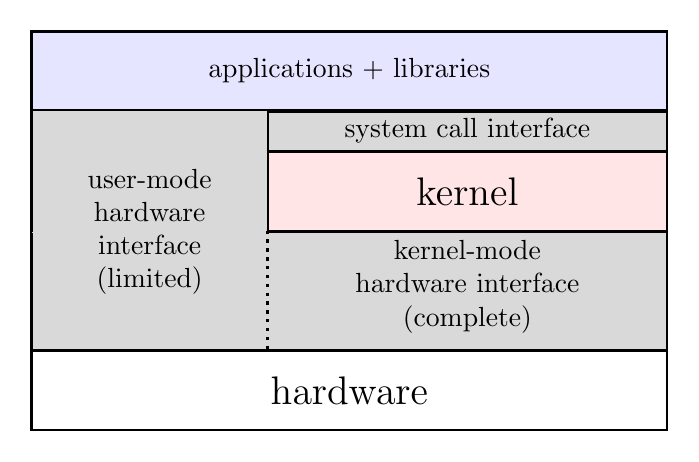
\begin{tikzpicture}
\tikzset{
    user/.style={fill=blue!10},
    iface/.style={fill=black!15},
    kernel/.style={fill=red!10},
    hardware/.style={},
}
% FIXME: show standard libraries/etc. can use HW directly
\matrix[matrix of nodes,
        inner sep=1pt, outer sep=0pt,
        row sep=-\pgflinewidth,
        column sep=-\pgflinewidth,
        nodes={draw,rectangle,inner sep=1pt,outer sep=0pt,thick,text width=8cm,align=center},
        ] {
    |[minimum height=1cm,alias=apps,user]| applications + libraries \\
    |[minimum height=0.5cm,alias=syscalls,iface,text width=5cm,xshift=1.5cm]| system call interface \\
    |[minimum height=1cm,alias=kernel,kernel,text width=5cm,xshift=1.5cm,font=\Large]| kernel \\
    |[minimum height=1.5cm,alias=hwIface,iface]| ~ \\
    |[minimum height=1cm,alias=hw,hardware,font=\Large]| hardware \\
};
\path[iface] (hwIface.north west) -- ++(3cm, 0cm) |- (apps.south west) |- (apps.south west) -- cycle;
\path[draw,very thick,black!15] ([xshift=3cm]hwIface.north west) -- (hwIface.north west);
\path[draw,thick] ([xshift=3cm]hwIface.north west) |- (apps.south west) |- (apps.south west) -- (hwIface.north west);
\path[draw,very thick,dotted] (kernel.south west) -- (kernel.south west |- hw.north);
\node[align=center] at ([xshift=1.5cm,yshift=0cm]hwIface.north west) {
    user-mode \\
    hardware \\
    interface \\
    (limited)
};
\node[anchor=north,align=center] at (kernel.south) {
    kernel-mode \\ hardware interface \\ (complete)
};
\end{tikzpicture}
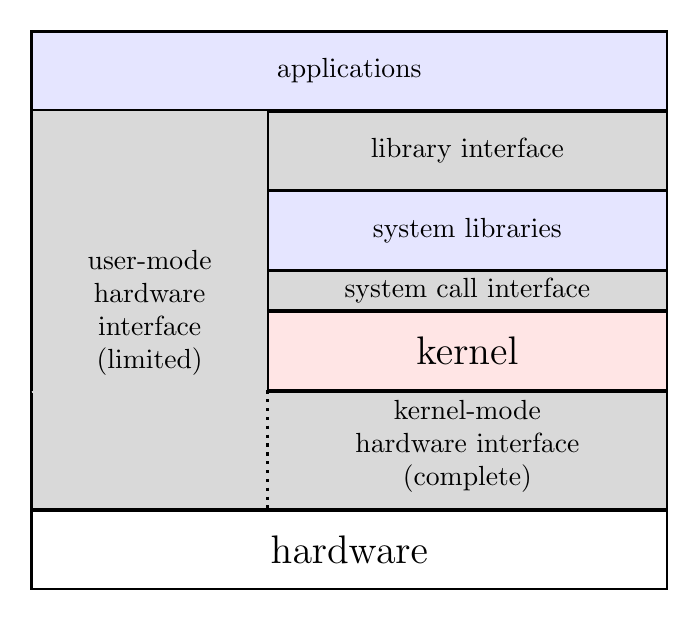
\begin{tikzpicture}
\tikzset{
    user/.style={fill=blue!10},
    iface/.style={fill=black!15},
    kernel/.style={fill=red!10},
    hardware/.style={},
}
% FIXME: show standard libraries/etc. can use HW directly
\matrix[matrix of nodes,
        inner sep=1pt, outer sep=0pt,
        row sep=-\pgflinewidth,
        column sep=-\pgflinewidth,
        nodes={draw,rectangle,inner sep=1pt,outer sep=0pt,thick,text width=8cm,align=center},
        ] {
    |[minimum height=1cm,alias=apps,user]| applications \\
    |[minimum height=1cm,alias=syslibiface,iface,text width=5cm,xshift=1.5cm]| library interface \\
    |[minimum height=1cm,alias=stdlib,user,text width=5cm,xshift=1.5cm]| system libraries \\
    |[minimum height=0.5cm,alias=syscalls,iface,text width=5cm,xshift=1.5cm]| system call interface \\
    |[minimum height=1cm,alias=kernel,kernel,text width=5cm,xshift=1.5cm,font=\Large]| kernel \\
    |[minimum height=1.5cm,alias=hwIface,iface]| ~ \\
    |[minimum height=1cm,alias=hw,hardware,font=\Large]| hardware \\
};
\path[iface] (hwIface.north west) -- ++(3cm, 0cm) |- (stdlib.south west) |- (apps.south west) -- cycle;
\path[draw,very thick,black!15] ([xshift=3cm]hwIface.north west) -- (hwIface.north west);
\path[draw,thick] ([xshift=3cm]hwIface.north west) |- (stdlib.south west) |- (apps.south west) -- (hwIface.north west);
\path[draw,very thick,dotted] (kernel.south west) -- (kernel.south west |- hw.north);
\node[align=center] at ([xshift=1.5cm,yshift=1cm]hwIface.north west) {
    user-mode \\
    hardware \\
    interface \\
    (limited)
};
\node[anchor=north,align=center] at (kernel.south) {
    kernel-mode \\ hardware interface \\ (complete)
};
\end{tikzpicture}
\end{document}
